\documentclass[a4paper,12pt,twoside,final]{report}

\usepackage[utf8]{inputenc}
\usepackage[english]{babel}
\usepackage[T1]{fontenc}

\usepackage{times}  
\usepackage{amsmath}
\usepackage{amssymb}
\usepackage{graphicx}
\usepackage{theorem}
\usepackage{latexsym}
\usepackage{geometry}
\usepackage{float}
\usepackage{tabularx}

\geometry{
 margin=20mm
} 

%To-Do
%1. Add pressure picture to results
%2. Explain variabels in equations
%3. Explain pictures
%4. Infoga referenser i texten, även till bild för SPH
%5. Bättre manual
%6. Skriv mer på resultat, mer siffror

%extra, se till att exe fil fungerar på pc

\renewcommand{\contentsname}{Table of contents}
\begin{document}

\pagestyle{plain}

%----------------------------- Front matter of the document

\title{Smoothed Particle Hydrodynamics in Zero Gravity}
\author{Oscar Westberg, Teodor Vik, Mikael Zackrisson, Anton Österblad}
\maketitle

\thispagestyle{empty}
\newpage{}

\setcounter{page}{2}
\renewcommand{\abstractname}{Summary}
\begin{abstract}
This project was part of the course TNM085, Modeling project at Linköping University. Groups were able to choose their own research topics and simulate a physical model. This report describes a simulation of a system using Smoothed Particle Hydrodynamics (SPH) in both zero gravity and under the effect of gravity. \\

\noindent The result is a program able to simulate a 2D SPH particle system with water-like attributes, up to 900 particles are simulated simultaneously. The program uses C++ and OpenGL to simulate this system using Navier-Stokes in real time.
\vfill
\end{abstract}
\newpage{}

\tableofcontents  % chapter with the table of contents
\addtocontents{toc}{\protect\thispagestyle{empty}}
\listoffigures    % chapter with the list of figures
\addtocontents{lof}{\protect\thispagestyle{empty}}
\listoftables     % chapter with the list of tables
\addtocontents{lot}{\protect\thispagestyle{empty}}


%----------------------------- Body of the document
\chapter{Introduction}


%----------------------------- Background
\section{Background}
Fluid simulation is a popular tool in computer graphics and it is often used to simulate liquid, smoke and explosions. Depending on the quality requirements fluid simulations can be extremely time-consuming animations or simple real-time particle systems. Since particle system is a good way to simulate a complex effect it is very popular amongst developers and thus there are a lot of information to find about the subject. The report is based on Smoothed Particle Hydrodynamics, which is one of the most popular techniques when creating a fluid.


%----------------------------- Purpose
\section{Purpose}
The purpose of this project is to, based on mathematical models and physical formulas, perform a simulation of water in both earth like conditions and in zero gravity. The simulation shall be displayed graphically in real-time.


%----------------------------- Physical systems
\chapter{Physical systems}
There are several techniques for simulating a fluid. The most common techniques are based on the Navier-Stokes equations which describes the flow of fluids. To practically use the Navier-Stokes equations it is common to make some simplifications in which some properties are assumed to be constant. There are two fundamental approaches on how to implement the Navier-Stokes equations; the Eulerian method and the Lagrangian method. Both are widely used in computer graphics. \\

\noindent The Eulerian method uses a grid-based system, in which each grid point has fluid properties, like velocity, density, pressure, etc., but the points never move.
The Lagrangian method is based on a collection of particles that, in addition to the fluid properties, has a position and can move.


%----------------------------- Navier-Stokes
\section{Navier-Stokes equations}

Navier-Stokes equations describe the motion of fluid substances as a result of forces. \\

\begin{equation}
\frac{\partial \overrightarrow v}{\partial t} + ({\overrightarrow v}\cdot{\overrightarrow \nabla}){\overrightarrow v} = \frac{-\overrightarrow \nabla p}{\rho_m} + \frac{\mu}{\rho_m}{ \nabla^2}{\overrightarrow v} + \frac{\overrightarrow f_{ext}}{\rho_m}
\label{e1}
\end{equation}

\noindent$\rho_m$ = mass density\\*
$v$ = velocity\\*
$\nabla$= gradient\\*
$p$ = pressure\\*
$f_{ext}$ = external force\\*
$\mu$ = viscosity\\*

\noindent Navier-Stokes equations describe the motion of fluid substances as a result of forces. The forces are based on the physical quantities of the fluid (velocity v, mass density p and pressure) and also viscosity and external forces. Equation \ref{e1} describes the conservation of momentum, and basically it is Newton’s second law for a fluid.\\


%----------------------------- SPH
\section{Smoothed Particle Hydrodynamics}
Smoothed Particle Hydrodynamics (SPH) is a Lagrangian method that divides the fluid into a set of particles. Mass-density, pressure, etc. are estimated using SPH approximations. The properties of a SPH-particle is affected by other particles that lie within a certain “smoothing” distance, thus affected only by its neighbours. Any desired scalar quantity can be determined for each particle by weighting that quantity from neighboring particles with a “kernel function”. \\

\begin{figure}[h]
\begin{center}
    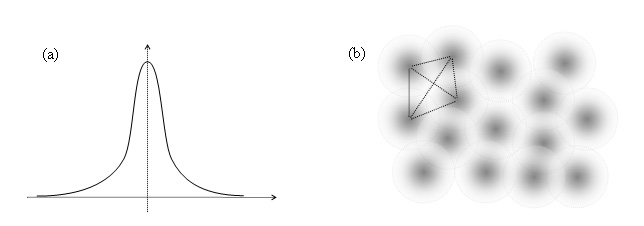
\includegraphics[width=11cm]{figs/sph.jpg} 
\end{center}
\caption{Smoothed Particle Hydrodynamics}
\label{model_block}
\end{figure}

\noindent An SPH simulation involves repeating these steps as time advances:
\begin{enumerate}

\item Compute density at each particle. \\ \\
\noindent The density will be calculated using the smoothing function (smoothing kernals).
\begin{equation}
{\rho_s}{(\overrightarrow r_j)} {\approx} {\sum_i}{w(\overrightarrow r_{ij})}
\label{e3}
\end{equation}

\item Compute pressure from density. \\ \\
\noindent The pressure can be approximately calculated using the density. k is a constant T.
\begin{equation}
{p_i} = {k(\rho_i -\rho_o)}
\label{e4}
\end{equation}

\item Compute forces from pressure gradients. \\ \\
\noindent Forces come from differences in pressure between two points (pressure gradients).
\begin{equation}
{\nabla p(\overrightarrow r_j)} =  {\rho_j}{\sum_j}(\frac{p_i}{\rho_i^2}+\frac{p_j}{\rho_j^2}){\nabla w(\overrightarrow r_{ij})}
\label{e5}
\end{equation}
\noindent $r_j$ and $r_i$ are two different points, $r_{ij}$ is the difference between them. \\
\noindent $\nabla w$ is a gradient calculation using the smoothing function.

\item Compute viscosity.
\begin{equation}
\frac{\mu}{\rho_i}{ \nabla^2 v_i} \approx \frac{\mu}{\rho_i}{\sum_j}(\frac{v_j - v_i}{p_j}){\nabla^2 w(r_{ij},h)}
\label{e6}
\end{equation}

\item Compute external forces. \\
\noindent Laws of gravity $F_{gravity}=\rho_i \cdot g$

\item Apply those forces to move particles. \\
\noindent In order to advance the particles we calculate the equations below every time we change the particles’ position.
\begin{equation}
{a} = {(-\nabla p(\overrightarrow r_j) + \frac{\mu}{\rho_i}{ \nabla^2 v_i} + g)}
\label{e7}
\end{equation} \\

\noindent \begin{equation}
{v} = {v + \Delta t \cdot a}
\label{e8}
\end{equation}
%pos = pos + TIME_STEP*v;

\end{enumerate}


%----------------------------- Implementation
\chapter{Implementation}

%----------------------------- Matlab
\section{Matlab}
A simple version of the model was simulated in MATLAB in order to test the theory behind the system as this eliminated the chances of any potential errors being caused by the rendering or implemented functions. The calculations was performed in the order that was previously described.

%----------------------------- OpenGL
\section{OpenGL}
The particle system’s functionality was tested in MATLAB, however the final product was created in C++. The program uses the libraries glm, glew, glfw, OpenGL and standard C++ functionality to render and simulate the particle system. From the main loop the program first checks for input, then updates the particle’s properties and then render the scene mainly by using a fragment shader. \\

\noindent Since only the closest neighbors of each particle will have an effect on its behavior it’s unnecessary to calculate the effect on every particle for each particle. This gives $N^2$ calculations. The performance was improved by using spatial subdivision. A uniform grid subdivides the simulation space into a grid of uniformly sized cells. This means that the the force for a given particle can be calculated by only comparing it with all its neighbors within a certain radius. \\

\noindent To ensure the rendered scene looks like water instead of a collections of dots the technique metaballs was implemented. A metaball emits an electric field according to the formula: $[f(x,y) = 1.0 / (x^2 + y^2)]$ \\

\noindent  If the accumulated contribution of several metaball fields reaches a certain threshold, the shader renders the color blue. The metaball technique makes the entire particle system look like a fluid.

\begin{figure}[H]
\begin{center}
    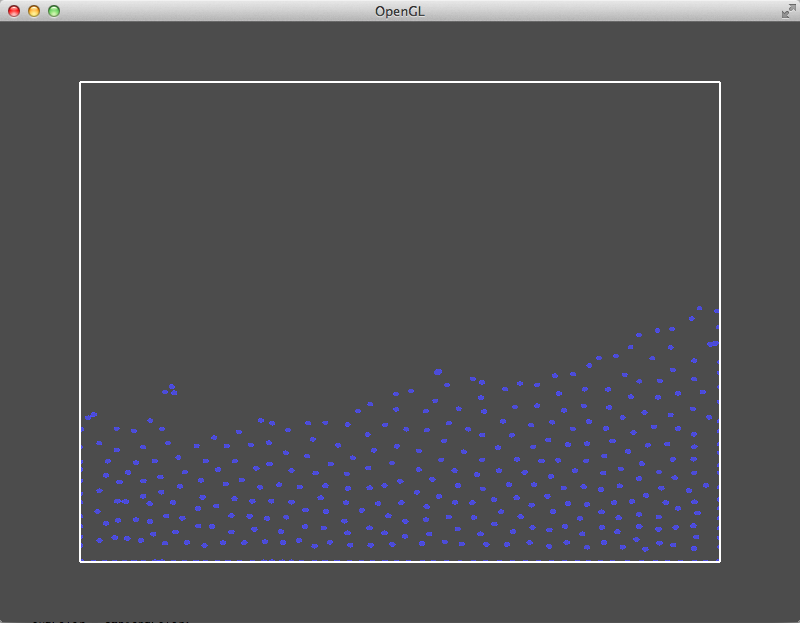
\includegraphics[width=11cm]{figs/image_2.png} 
\end{center}
\caption{Running the program without metaballs activated}
\label{model_block}
\end{figure}



%----------------------------- Result
\chapter{Result}

\begin{table}[h]
  \centering
  \caption{SPH parameters from Matlab simulation}
  \label{Matlab table}
    \begin{tabularx}{\textwidth}{| X | X | X |}
    \hline
    SPH parameters & Water & Yoghurt \\ \hline
    Particle mass & 0.013 & 0.014 \\ \hline
    Ideal density & 1000 & 1050 \\ \hline
    Viscosity constant & 3.5 & 20.0 \\ \hline
    Stiffness & 3.0 & 5.0 \\ \hline
    \end{tabularx}
\end{table}

\noindent The end product is an interactive program simulating a customizable amount of particles in either zero gravity or with gravity. The particle system is rendered in 2D in a window. Up to 900 particles run at full speed, it is also possible to change shader by pressing “s”. The shader with black water and red transparent squares displays the particles’ pressure. \\

\begin{figure}[H]
\begin{center}
    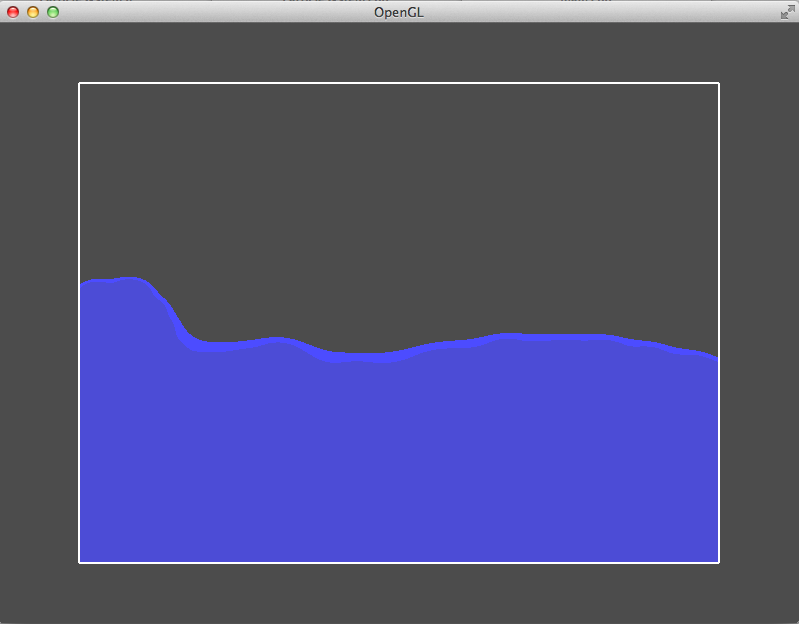
\includegraphics[width=11cm]{figs/image_1.png} 
\end{center}
\caption{Running the program with metaballs}
\label{model_block}
\end{figure}



%----------------------------- Conclusion and discussion
\chapter{Conclusion and Discussion}

Matlab was a great tool to test if the implementation of the physics for the system was correct. Since Matlab shows the correct output there were never any doubts that if something went wrong it was because of miscalculations and not how the system was drawn. However when all code for the system was implemented and the search for correct variables began OpenGL was better to use because it was much faster. The fast transition between Matlab and OpenGL was possible because we had separated the group into working with Matlab and OpenGL simultaneously. \\

\noindent There are a lot of articles about which variables to use when simulating water. However these have been guidelines and not the final values in our simulation since they did not provide us with a satisfying result. After tweaking the system we now think it behaves like water. \\

\noindent The initial idea of the program was to render water in 3D and to use advanced shaders to create a realistic look. The final result however is in only two dimensions. By adding a third dimensions it will drastically increase the shear number of particles and it was decided to stick with two dimension in the final version because of the performance restrictions of the system. The calculations are basically the same if a third dimension is added and will not be difficult to add in terms of coding. \\

\noindent There are several improvements to be made, for instance by introducing multi-core calculations on the CPU or making calculations on the GPU instead. \\

\noindent C++ is well known for being a fast programming language and was an obvious choice to start, in retrospect it was still a good choice to use C++. While the final product does not have 3D functionality, any other choice of programming language would most likely not reach the same level of speed with the team’s current programming proficiency. \\

\noindent OpenGL is a vital part of drawing in 3D and was a must in the project’s initial phase. Since the final product only uses 2D rendering other drawing libraries such as SFML and SDL would have been viable. The group did however want to learn OpenGL.



%-----------------------------

%\bibliographystyle{vancouver}
%\bibliography{refs/references}

%\addcontentsline{toc}{chapter}{References}
%\pagestyle{empty}
%\appendix
%\cite{auer08}
%\cite{kelager06}

%----------------------------- Bibliography

\begin{thebibliography}{11}

  \bibitem{auer08}
  Auer, S.
  \emph{Realtime Particle-Based Fluid Simulation}.
  Computer Graphics and Visualization,
  October 4th,
  2008.
  
  \bibitem{kelager06}
  Kelager, M.
  \emph{Lagrangian Fluid Dynamics Using Smoothed Particle Hydrodynamics}.
  Department of Computer Science, University of Copenhagen,
  January 9th,
  2006.

\end{thebibliography}

\newpage


%----------------------------- Attachments
\appendix
\chapter{Manual}
Manual, how to run the program and hardware requirements. \\
\noindent The easiest way to run the program is to execute the runnable file included with this file. It is also possible to use the source code to create a new executable but that requires linking of glfw, glm and glew. Make sure all the shader files are included in the same folder as the runnable file, another requirement is hardware supporting OpenGL 3.3 and above.

\end{document}